\documentclass{article}
\usepackage[utf8]{inputenc}

\title{Clear Sky Selection}
\author{Peter Shaffery, \rojo{Aron Habte, SRRL, Marcos Netto}, Venkat Krishnan}
\date{Feb 2020}
\usepackage[margin=1in]{geometry}
\usepackage{xcolor}
\usepackage{graphicx}

\usepackage[citestyle=numeric,backend=biber,natbib]{biblatex}
\bibliography{ref.bib}

\newcommand{\rojo}[1]{{\color{red} #1}}

\begin{document}
\maketitle
\section{Introduction}
The effect of distributed, photovoltaic (PV) generators on the power grid is rapidly becoming a key issue in grid management. PV generation can have substantial effects on the daily load observed at many levels of grid organization (consumer, distribution, or transmission). Effective integration of these elements and safe management of the grid is greatly enabled by accurate forecasting of their output \citep{m_coddinton_grid-integrated_2016,noauthor_visibility_2017}. Particularly at the distribution level, short-time forecasting of ramps in PV generation can improve grid stability and flexibility \citep{noauthor_coordination_2017}. Besides detailed PV site information, accurate forecasting of PV generation requires an accrurate, high-resolution solar resource forecasts, from which PV generation follows well-understood principals and can be straightforwardly modelled.

Nevertheless high-resolution, accurate solar forecasts are difficult to produce at the time-scales required by grid managers. Numerical weather forecasting, while generally having high accuracy, often cannot operate operate at the spatial and temporal resolutions necessary to precisely model PV generation due to constraints in both data availability and computational power \citep{diagne_review_2013,sengupta_best_2015}. Similarly, satellite observations tend to operate at spatial scales greater than is needed for high-quality solar resource forecasts. Therefore the development of cheap, scalable weather sensors, which can provide multiple channels of weather data (eg. not just solar irradiance intensity, but also cloud and wind conditions) are desirable \citep{summers_sensing_nodate}. One technology which is being explored as an avenue to develop such a sensor are Total Sky Imagers (TSIs, also denoting "Total Sky Images").

TSIs are high-resolution, fish-eye cameras with a 180-degree field of vision. These cameras provide a complete snapshot of the sky at a relatively high time resolution (up to 30 seconds). By combining TSIs with image processing and data-driven modelling techniques, it may be possible to produce a variety of data products which can be useful to solar resource forecasts \citep{chow_intra-hour_2011,ghonima_method_2012}. A common technique often used with TSIs is correlation-based movement detection \citep{huang_correlation_nodate}. This algorithm takes two time-adjacent images and, via a discrete Fourier Transform, finds their spatial correlation, and thus a translation vector between the images. This vector is then taken to estimate the wind conditions, and is used to ``push-forward" the most recent TSI, generating a forecasted cloud image. More sophisticated variants of this approach achieve higher accuracy by performing this operation locally, estimating a wind vector field \citep{hamill_short-term_1993,marquez_intra-hour_2013,magnone_cloud_2017}.

Either using correlation forecasting or other methods, a key step to make TSIs useful for solar resource forecasting is the procurement of a ``clearsky dictionary" (CSD) \citep{ghonima_method_2012}. The CSD refers to a collection of images or pixels representing cloudless sky, indexed by time of day, solar angle, or both. This provides a baseline of cloudless pixels which can be compared against to classify a given observed pixel as containing clouds, sun, or clearsky. Unfortunately, CSDs are often hand-labelled, which can be particularly time-consuming and does not scale. Automation of this process is still in early stages, and requires hand-tuning \citep{pawar_detecting_2019}.

In this paper we propose an unsupervised, automatic approach to compiling CSDs. We define a clear-sky pseudo-index, based on the Red-Blue Ratio (RBR) of a given TSI \citep{dev_rough-set-based_2017}. By calculating this pseudo-index for each image in a dataset, and then minimizing it for each of a sequence of time periods (here defined to be the hours of a day), each time period can be assigned a clear-sky image (if one is present in the dataset). We will demonstrate the performance of this approach on a dataset of TSIs provided by the NREL Solar Radiation Research Laboratory (SRRL), and compare it to ground-truth measurements of true clear-sky index. 


\section{Data}
TSIs were taken using an All-Sky Imager (ASI) {\color{red}model XXXXX and info}.  Each image in the dataset is an $n \times n \times 3$ data volume denoted $G_{(k,m)}$ where $k$ indexes the day, $m$ indicates its time, and $n=1536$ is the resolution of the TSI along one side. Each $n \times n$ layer of the volume represents either the red, green, or blue channel of image $k$. Elements of the volume take integer values between $0$ and $255$.

Because of the high resolution of the TSIs ($1536\text{px} \times 1536\text{px}$) some thought was given to data manipulation procedures. The total dataset is about 8.4GB in size, and so loading it entirely into memory is unwieldy. To this end, data processing proceeded in multiple stages. TSIs were first unpacked into a directory structure explicitly ordered by image timestamp; a  TSI taken by camera 11 at 07:00:00am April 2nd, 2019 was placed in directory branch \texttt{11/2019/04/02/070000.jpeg}. This simplified the scripting logic of matching images to unique timestamps. Images were then batch processed at the day-level, and a Pandas DataFrame of their statistics was calculated for each day. Finally, these dataframes were combined into one which could be processed to calculate, for each TSI, a clear sky pseudo-index.

\section{Methods}
The day-level batch processing consisted of a series of operations which converted the image into a vector of summary statistics corresponding to the image's timestamp. First, we computed the Red-Blue Ratio (RBR) for each non-zero pixel. This reduced the image from an $n \times n \times 3$ data volume to an $n \times n$ array. Let $R_{k,m}$ and $B_{k,m}$ denote the Red and Blue channels of an image $G_{(k,m})$, where $k$ denotes the day the images was taken on, and $m$ denotes the time it was taken at. Then for each each pixel (indexed by $(i,j)$) we computed the RBR:
\begin{equation}
    \rho_{k,m}^{(n,l)} = \frac{ R_{k,m}^{(n,l)} }{ 1+B_{k,m}^{(n,l)} }
\end{equation}

Next the RBR images were cropped. This removed all non-sky context (eg. a timestamp in the corner, surrounding landscape or buildings) as well as some highly distorted sky content due to fish-eye effects. This was done by multiplying the the RBR image elementwise by a ``crop mask" mask, an $n \times n$ array which is 1 for all indices inside a circle of radius $R$ centered at the pixel $(\floor{n/2},\floor{n/2})$), and $0$ otherwise. The radius was set to $R=.98\frac{n}{2}$, which was chosen by visual inspection.

Having converted the images to RBR and cropped them, we next calculated the image statistics using a ``histogram approach" \citep{gonzales_digital_1992}. This discarded all spatial information, treating the image only as a histogram of pixel values for which image-level statistics were be computed. These were $m_{k,m} = \text{E}[\rho_{k,m}]$ (the mean RBR) and $\rho$ and $s_{k,m} = \sqrt{\text{Var}[G_{k,m}]}$ (the standard deviation of RBR). 

From these we calculated the clear-sky pseudo-index, defined as:
\begin{equation}
    \label{eq:csi}
    \gamma_{k,m} = m_{k,m}*s_{k,m}
\end{equation}

The pseudo-index can be interpreted by observing that $s_{k,m}$ corresponds to RBR contrast; the visual range of the image pixels. When contrast is low, images are homogenous which is characterstic of images showing only clear-sky. However, images showing complete cloud cover also have homogenous RBR, and therefore we jointly penalize $m_{k,m}$, corresponds to choosing images with  high blue-content. This selects against images with large amounts of white, due to high cloud content. 

Having calculated $\gamma_{k,m}$ for each image, we can now compile the CSD. This was done by simply merging all image statistics calculated within each day into a single dataframe, and then for each hour finding the minimum pseudoindex value. However, for larger datasets a MapReduce approach could be used to reduce the computational burden. The presentation here assumes a single dataset to minimize over.    
Let $h(m)$ be the function which takes a time $m$ and rounds it the most recent hour (so $h(\text{07:15:00}) = h(\text{07:45:00}) = 7$, etc.). 
Let the set $H_{\eta} = \{ \gamma_{k,m} | h(m) = \eta \}$ denote the collection of all pseudoindices $\gamma_{k,m}$, over all days $k$, and where the time $m$ is such that $h(m) = \eta$. The CSD is defined as the set of triples:
\[
\text{CSD} = \{(1,k_1^*,m_1^*),...,(\eta,k_{\eta}^*,m_{\eta}^*)\}
\]
Where the first element of the triple indicates the hour of the day, and the second and third indicate the day and timestamp of the clearsky image which is the dictionary element correspond to hour $\eta$. $k_{\eta}^*$ and $m_{\eta}^*$ are found by:    
\[
(k_{\eta}^*,m_{\eta}^*) = \text{argmin}_{k,m} \gamma_{k,m} \in H_{\eta}
\]

\section{Results}
We assess the performance of our algorithm in several ways. First, we visually examine the images selected as clear-sky (Fig. \ref{fig:csd_ex}). The CSD appears to perform well: all images selected contain few clouds, particularly around the solar region. The heuristic of choosing low-contrast images with a low RBR appears effective for selecting images with high blue content. 

\begin{figure}[h]
    \centering
    \begin{tabular}{cc}
    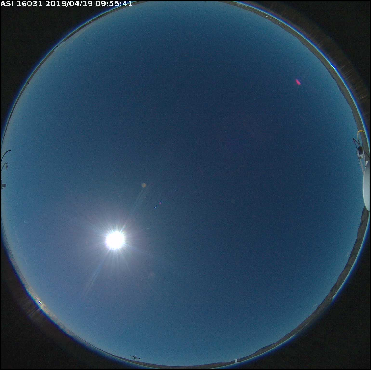
\includegraphics[scale=.5]{Figures/ex1.png} & 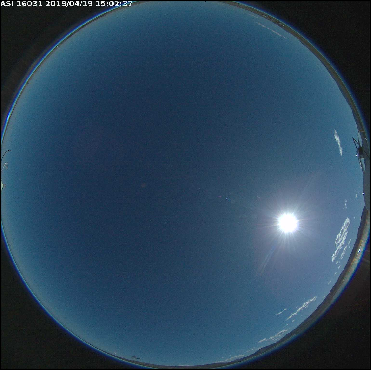
\includegraphics[scale=.5]{Figures/ex2.png} &\\
    (a) & (b) \\
    \end{tabular}
    \caption{Two example images selected for inclusion in the CSD. Image (a) represents clear-sky at 10:00MST, whereas (b) represents clear-sky at 16:00MST.}
    \label{fig:csd_ex}
\end{figure}

In addition to visual inspection, we can look at how our clear-sky pseudo-index and resulting CSD relates to a true clear-sky index. To do this we merge the dataset of images with a dataset of clear-sky indices provided by the NREL Solar Radiation Research Laboratory (SRRL). Here the true clear-sky index was defined as:
\[
g_{t} = \frac{d_t}{E_t}
\]
Where $d_t$ is the amount of Direct Normal Irradiance (DNI) measured by a pyranometer sited close to the ASI at time $t$, and $E_t$ is the estimated Extraterrestrial Direct Irradiance (EDI) at time $t$. That is, $g_t$ is the Direct Clear Sky Index (DCSI), the amount of solar irradiance received on the ground as a ratio of all initially inbound irradiance. By matching $g_t$ to the timestamp of each image within the CSD we can look at whether the CSD images truly represent clear-sky.

Fig \ref{fig:dcsi_hist} shows the histogram of DCSI values for the entire dataset, as well as for the CSD images. We see that the TSIs selected for inclusion to the CSD have some of the highest DCSI values possible for the dataset (all are withing the 80th percentile of DCSI values, and most are in the 90th percentile). We can refine this comparison by plotting the DCSI of the images in our CSD achieve against the the highest possible hourly DCSI (Fig. \ref{fig:dcsi_perf}). That is, for each hour $\eta$ we compare the value of $\gamma_{k_{\eta}^*,m_{\eta}^*}$ to the maximum of $g_{t)}$ where $t$ ranges over all timepoints such that $h(t) = \eta$. We see that, in general our CSD values perform quite well, with most images falling only slightly short of best-possible choice. Together these plots suggests that our model is well-calibrated, ie. that the images chosen for inclusion are good choices, relative to the ground-truth.

Interestingly, despite the fact that our algorithm accurately selects clear-sky images, our clear-sky pseudoindex is only weakly predictive of DCSI overall (Fig. \ref{fig:cpsi_dcsi}). While linear regression between $g_t$ and $\gamma_t$ indicates that a relationship does exist ($p<.05$), there is substantial variation in DCSI not explained by changes in the pseudo-index ($R^2=.14$). This may be because the pseudo-index is based on the entire image, and will change if clouds are present far outside the solar region. These clouds will have little impact on the DNI however, and thus little impact on DCSI. While the pseudo-index is still effective at selecting clear-sky images, if a tighter relationship with DCSI is desired pre-cropping the image to reflect only the solar region may be needed.

\begin{figure}[h]
    \centering
    \begin{tabular}{cc}
    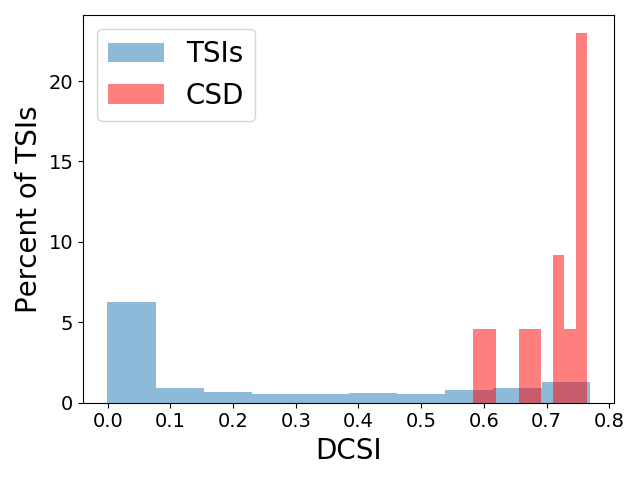
\includegraphics[width=.5\textwidth]{Figures/csd_dcsi_hist.png} & 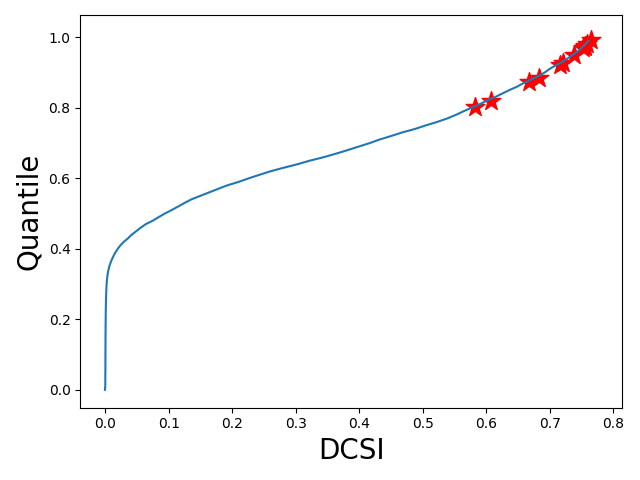
\includegraphics[width=.5\textwidth]{Figures/csd_dcsi_quants.png}  \\
       (a)  & (b) \\
    \end{tabular}
    \caption{(a) Histogram of true DCSI for all TSIs (blue) as well as for images in the CSD (red). Histogram is scaled to percentage of dataset, rather than raw counts. (b) Quantile plot of all DCSI values, with the DCSI corresponding to images in the CSD marked with a red star.}
    \label{fig:dcsi_hist}
\end{figure}

\begin{figure}[h]
    \centering
    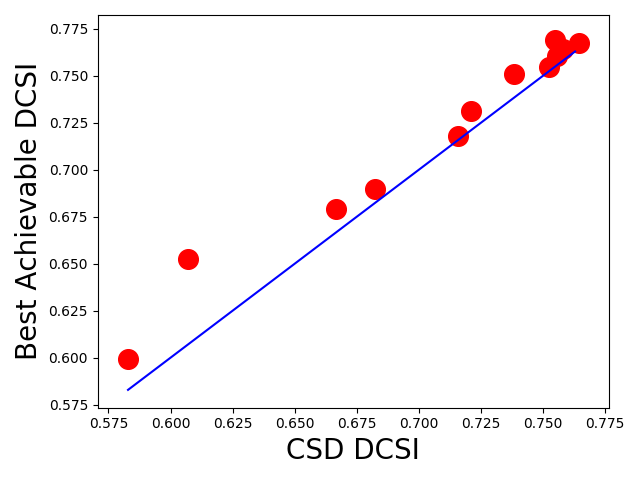
\includegraphics[scale=.7]{Figures/csd_dcsi_perf.png}
    \caption{The best achievable DCSI for each hour within our CSD, plotted against the actual DCSI achieved by the CSD for that hour (red points). The blue line indicates perfected equality, when points are high above this line it indicates that our algorithm underperformed relative to the ground truth.}
    \label{fig:dcsi_perf}
\end{figure}

\begin{figure}[h]
    \centering
    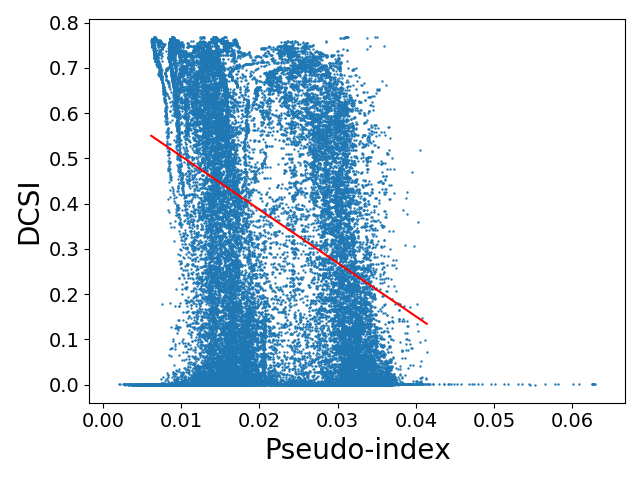
\includegraphics[scale=.7]{Figures/cspi_dcsi_scatter.png}
    \caption{Scatterplot of true DCSI against our pseudo-index for all TSIs in the dataset. A best-fit line between DCSI and the pseudo-index was found for all points where $\text{DCSI}>0$ and plotted in red. }
    \label{fig:cpsi_dcsi}
\end{figure}


\section{Discussion}
We have proposed a method for automated construction of a CSD and demonstrated its performance on an example dataset. Our proposal accurately selects clear-sky images, as measured by the DCSI, with the chosen images having some of the the highest DCSI values in the dataset. Although we do not achieve the highest possible DCSI in all cases, in general our chosen images are close to the best possible choice.   

Despite our CSD images representing some of the clearest sky images, our pseudoindex was overall not strongly predictive of the true DCSI. This suggests that our algorithm may struggle to be generalized if more clear-sky images are desired. This may be improved by including some spatial information in our pseudoindex. Either pre-cropping the images to include only solar pixels, or weighting the image mean-RBR by pixel distance from the solar region may improve the relationship between pseudoindex and DCSI. 

A useful feature of our approach is that it requires no parameter tuning besides the cropping width of the images, which is straightforward to select. Our method is therefore agnostic to the TSI type and location, as it simply selects the ``best" candidates from the total dataset. This is desirable, as it increases the scalability of a TSI-based sensor for solar resource forecasting. All that is required for our algorithm to work is for the training data to contain actual clear-sky images.

\newpage
\printbibliography
\end{document}
